\documentclass{beamer}
\usepackage{listings}
\lstset{
%language=C,
frame=single, 
breaklines=true,
columns=fullflexible
}
\usepackage{subcaption}
\usepackage{url}

\newcommand{\fbrack}[2]{\genfrac{(}{)}{}{}{#1}{#2}}
\usepackage{tikz}
\usepackage{pgfplots}
\pgfplotsset{compat=1.17}
\usepackage{tkz-fct}
\usepackage{mathrsfs}
\usepackage{txfonts}
\usepackage{tkz-euclide} 
\usetikzlibrary{calc,math}
\usepackage{float}
\newcommand\norm[1]{\left\lVert#1\right\rVert}
\renewcommand{\vec}[1]{\mathbf{#1}}
\providecommand{\pr}[1]{\ensuremath{\Pr\left(#1\right)}}
\usepackage[export]{adjustbox}
\usepackage[utf8]{inputenc}
\usepackage{amsmath}
\usetheme{Boadilla}
\title{Performance Analysis of Digital Communications over Rician-TWDP Channels}
\author{Ojjas Tyagi - MA20BTECH1102/CS20BTECH11060}
\begin{document}
\begin{frame}
\titlepage
\end{frame}
\section{Introduction}
\begin{frame}
\frametitle{Introduction}
\begin{block}{Contents}
This  paper presentation explores the  conceptual  behavior  of  digital  communication  for  the  composite  Rician-Two  Wave  Diffuse Power (TWDP) fading-shadowing model. Here, small scale  fading  is  attributed  by  the  Rician  channel,  whereas  shadowing  effects  are  modeled  by  TWDP.\\ We explore various statistical characteristics such as PDF,CDF and Outage Probability. 
\end{block}
\end{frame}
\section{Definitions}
\subsection{functions}
\begin{frame}{Function Definitions}
\begin{block}{Gamma Function \(\Gamma(x)\)}
Gamma function is defined as 
\begin{align}
    &\Gamma(x)=\int_0^\infty t^{x-1} \exp(-t) dt \\ \nonumber
    &\Gamma(n)=(n-1)! \text{\quad when n is a positive integer}
\end{align}
\end{block}
\begin{block}{Gen. Hypergeometric Function \(_{p} F_q\)}
A generalized hypergeometric function \(_{p} F_q\) is given by 
\begin{align}
    &_{p} F_{q} (a_1,...,a_p;b_1,...b_q;z)=\sum_{n=0}^{\infty} \frac{(a_1)_{n}...(a_p)_{n}}{(b_1)_{n}...(b_q)_{n}} \times \frac{z^n}{n!} \label{hypergeo}\\ \nonumber
    &\text{where \((x)_n\) stands for pochhammer symbol i.e}\\ \nonumber 
    &(x)_n =\frac{\Gamma(x+n)}{\Gamma(x)}=x(x+1)(x+2)...(x+n-1)
\end{align}
\end{block}
\end{frame}
\begin{frame}
\begin{block}{Modified Bessel function of first kind and zero order \(I_0\)}
 Bessel differential equation which is given by
\begin{align} \nonumber
    x^{2}y" + x y'-(x^{2} +n^{2})=0
\end{align}
which has the linearly independent solutions \(I_n(x)\) and \(K_n(x)\) which are the modified bessel functions of the first and second kind respectively,where n is the order\\
when n is real \(I_n(x)\) can be computed as 
\begin{align}
    I_n(x)=\fbrack{x}{2}^n \sum_{k=0}^{\infty} \frac{\fbrack{x^2}{4}^k}{\Gamma(n+k+1) k!} \label{bessel}
\end{align}
\end{block}
\begin{block}{Lower Incomplete Gamma Function \(\gamma(s,x)\)}
    \begin{align}
        \gamma(s,x)=\int_{0}^x t^{s-1} \exp(-t) dt
    \end{align}
\end{block}
\end{frame}
\subsection{useful terminology}
\begin{frame}{Some useful terms}
\begin{block}{Types of components}
\begin{enumerate}
    \item \textbf{Specular/LOS component } singular term with fixed magnitude and random phase which has direct line of sight with receiver is known as Specular component
    \item \textbf{Diffused component} Non specular component ,made of many waves each carrying power negligible to total average power,given by zero mean gaussian variables 
\end{enumerate}
\end{block}
\begin{block}{Processes in wireless communication}
\begin{enumerate}
    \item \textbf{Shadowing} Occurs when there is large obstacle between signal and receiver
    \item \textbf{Smallscale Fading} Power fluctuation for very short duration due to rapid interference of radio signals 
\end{enumerate}
Both of these are shown by fading models
\end{block}
\end{frame}
\section{model and statistics}
\subsection{PDF's}
\begin{frame}{System Model}
\begin{block}{Rician Multipath Fading}
In Rician case there is only 1 LOS component along with diffused component.PDF of fading is given by
\begin{align}
    f_{R} (r)=\frac{r}{P_1} \exp\left(-\frac{r^2}{2 P_1} - K_1\right) I_0 \left( r\sqrt{\frac{2K_1}{P_1}}\right) \label{rician}
\end{align}
here \\
R denotes magnitude of received complex envelope/fading amplitude,relates to amplitude of received signal\\
\({K}_1\) is Rician K factor = \({A^2}/{2P_1}\) where\\
\(A\) is magnitude of specular component  and\\
\(P_1\) is Mean squared voltage of diffused component\\
\(I_0\) is modified bessel function of first kind and zero order
\end{block}
\end{frame}
\begin{frame}
\begin{block}{TWDP shadowing}
  Two waves with diffuse power fading consist of two direct specular  components  along  with  diffused  components.The shadowing follows the TWDP distribution whose closely approximate PDF is given as\\
  \begin{align}
      & f_Y(y)=\frac{y}{2P_2} \sum_{j=0}^{1} \exp\left(\frac{-y^2}{2P_2}\right)
       \sum_{i=1}^{L} a_i \exp(-P_{2ij}) I_0\left( y \sqrt{\frac{2P_{2ij}}{P_2}}\right) \label{TWDP}
  \end{align}
  here\\
  \(P_2\) is mean squared voltage of diffused components\\
  \(K_2\) is TWDP K factor =\((A_1^2 +A_2^2)/{2P_2}\) where\\
  \(A_1\) and \(A_2\) are magnitudes of the two specular components\\
  \(P_{2ij}=K_2 \left(1+ (-1)^j \Delta \cos \left(\pi\left( \frac{i-1}{2L-1}\right)\right)\right)\)\\
  \(\Delta\) is relative strength of 2 LOS components =\(\frac{2 A_{1} A_{2}}{A_1^2 +A_2^2}\)\\
  \(L\) is order of approx TWDP and should be \(\geq \frac{1}{2} K\Delta\)
\end{block}
\end{frame}
\begin{frame}{}
   \begin{figure}
       \centering
       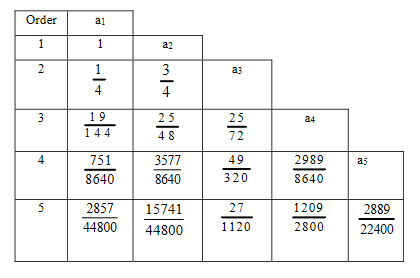
\includegraphics{Figures/Values of a_i.PNG}
       \caption{Values of \(a_i\)}
       \label{fig:my_label}
   \end{figure}
\end{frame}
\begin{frame}{Statistical Characteristics}
\begin{block}{Composite PDF}
We  studied  the  Rician  fading  channel  in  which  the  dominant  line-of-sight  component  is  subjected  to  TWDP shadowing. Using the concept of shadowing, the signal envelope, R, at receiver in a shadowed Rician-TWDP channel can be obtained by solving the conditional probability given as:
\begin{align}
    &f_R(r)=\int_0^\infty f_{(R|Y)} (r|y) f_Y(y) dy \label{composite}
\end{align}    
where 
\begin{align} 
    &f_{(R|Y)} (r|y) = \frac{r}{P_1} \exp\left(-\frac{r^2}{2 P_1} - K_1 y^2\right)
    I_0 \left( yr\sqrt{\frac{2K_1}{P_1}}\right) \label{rician-cond}
\end{align}
\end{block}
\end{frame}
\begin{frame}
\begin{block}{}
Now using eqns \eqref{TWDP},\eqref{composite} and \eqref{rician-cond} and , we get
\begin{align}
&f_R(r)=\frac{r}{2P_1P_2}\exp\left(\frac{-r^2}{2P_1}\right) \sum_{j=0}^{1} 
       \sum_{i=1}^{L} a_i \exp(-P_{2ij})  \times \\ \nonumber
       &\int_0^\infty y \exp \left( -y^2 \left(K_1+ \frac{1}{2P_2}\right)\right) 
        I_0 \left( yr\sqrt{\frac{2K_1}{P_1}}\right)  I_0 \left( y\sqrt{\frac{2P_{2ij}}{P_2}}\right) dy
\end{align}
now using \eqref{bessel} and the following identity
\begin{align}
    &\int_0^\infty x^{\mu -0.5}\exp(-\alpha x) I_{2\nu} (2\beta \sqrt{x})dx \label{int_1}\\ \nonumber
    &=\frac{\Gamma(\mu +\nu+0.5)}{\Gamma(1+2\nu)}\frac{\exp(\frac{\beta^2}{2\alpha})}{\beta \alpha^\mu} M_{-\mu,\nu}(\frac{\beta^2}{\alpha})\\ \nonumber
    &\text{where \(M_{k,m}(z)\) is defined as } \\
    &M_{k,m}(z)=\exp{(-0.5z)} z^{m+0.5} {}_{1} F_1(0.5+m-k;1+2m;z) \label{whit}
\end{align}
\end{block}
\end{frame}
\begin{frame}
\begin{block}{}
  Using \eqref{bessel},\eqref{int_1} and \eqref{whit} we get 
  \begin{align}
      &f_R(r)=\frac{r}{2P_1(2K_1P_2+1)}\exp\left(\frac{-r^2}{2P_1}\right) \sum_{i=1}^{L} a_i  \sum_{j=0}^{1} 
       \exp(-P_{2ij})  \times \label{f_R} \\ \nonumber
      &\sum_{v=0}^\infty \frac{\Gamma(v+1)}{(v!)^2}\left(\frac{P_{2ij}}{2K_1P_2+1}\right)^v {}_{1}F_{1}
      \left( v+1;1;\frac{K_1P_2r^2}{P_1(1+2K_1P_2)}\right)
  \end{align}
\end{block}
\end{frame}
\subsection{CDF ,SNR other results}
\begin{frame}{}
\begin{block}{Instantaneous SNR PDF derivation \(f_{\gamma}\)}
When  this  signal  is  passed  into  the  channel,  it  is  added  with  Gaussian Noise. As a result, the received instantaneous signal to noise power ratio is raised by \(R^2\),If we define instantaneous signal to noise power ratio per symbol as, \(\gamma=\frac{R^2 E_s}{N_0}\),then the pdf of the instantaneous SNR is given by using \eqref{f_R} and \(f_{\gamma}(\gamma) =\frac{f_R(\sqrt{\Omega\gamma/\bar{\gamma}})}{2\sqrt{\gamma\bar{\gamma}/\Omega}} \) , we get
\begin{align}
    f_{\gamma}(\gamma)=\frac{\Omega}{4P_1(2K_1 P_2)\bar{\gamma}} 
    \sum_{i=1}^{L} a_i  \sum_{j=0}^{1} 
       \exp(-P_{2ij}-\frac{\gamma\Omega}{2P_1\bar{\gamma}})  \times \label{f_gamma} \\ \nonumber
      \sum_{v=0}^\infty \frac{\Gamma(v+1)}{(v!)^2}\left(\frac{P_{2ij}}{2K_1P_2+1}\right)^v {}_{1}F_{1}
      \left( v+1;1;\frac{K_1P_2 \gamma\Omega}{P_1(1+2K_1P_2)\bar{\gamma}}\right)
\end{align}
where \(\bar{\gamma}\) is the average SNR and \(\Omega =E[R^2]\)\\
\(E_s\) is  the  energy  per  symbol\\
\(N_0\) is one-sided  power  spectral  density of AWGN
\end{block}
\end{frame}
\begin{frame}
\begin{block}{CDF derivation}
CDF is given by \(F_R(r)=\int_0^r f_R(a)da\), now using \eqref{hypergeo},\eqref{f_R} and the following idenitity
\begin{align}
     &\int_0^{u} x^m \exp(-\beta x^{n})dx =\frac{\gamma(v,\beta u^n)}{n\beta^v} \quad v=\frac{m+1}{n} \label{int_2}
\end{align}
Now we get CDF to be
\begin{align}
     &F_R(r)=\frac{1}{2(2K_1P_2+1)} \sum_{i=1}^{L} a_i  \sum_{j=0}^{1} 
     \exp(-P_{2ij})  \times \label{F_R}\\ \nonumber
    &\sum_{v=0}^\infty \frac{1}{(v!)^2}\left(\frac{P_{2ij}}{2K_1P_2+1}\right)^v
    \sum_{s=0}^\infty  \frac{\Gamma(v+s+1)}{s!\,\Gamma(s+1)} \gamma\left(s+1,\frac{r^2}{2P_1}\right)
\end{align}
\end{block}
\end{frame}
\begin{frame}
\begin{block}{n-moment derivation}
We can find the n\(^{th}\) moment by 
\begin{align}
    E[R^n]=\int_0^\infty r^n f_R (r)dr
\end{align}
Using \eqref{f_R} and identity given below
\begin{align}
    \int_0^\infty e^{-st} t^{b-1} {}_{1} F_{1}(a;c;kt)dt =\Gamma(b) s^{-b} {}_{2}F_{1}(a,b;c;\frac{k}{s})
\end{align}
now we get 
\begin{align}
    &E[R^n]=\Gamma(\frac{n}{2}+1) (2P_1)^{\frac{n}{2}} W^{(n)}(v,K_1,a_i,P_{2ij},P_2) \label{R^n} \\\nonumber
    &W^{(n)}(v,K_1,a_i,P_{2ij},P_2)=\frac{1}{2(2K_1P_2+1)} \sum_{i=1}^{L} a_i  \sum_{j=0}^{1} 
     \exp(-P_{2ij})  \times \\ \nonumber
    &\sum_{v=0}^\infty \frac{\Gamma(v+1)}{(v!)^2}\left(\frac{P_{2ij}}{2K_1P_2+1}\right)^v
    {}_{2}F_{1}\left(v+1,\frac{n}{2}+1;1;\frac{2K_1 P_2}{2K_1 P_2 +1}\right)
\end{align}
\end{block}
\end{frame}
\begin{frame}{}
\begin{block}{Mean}
Given by \(E[R]\) ,using n=1 in \eqref{R^n} we get
    \begin{align}
        E[R]=\sqrt{\frac{\pi P_1}{2}}W^{(1)}(v,K_1,a_i,P_{2ij},P_2) \label{mean}
    \end{align}
\end{block}
\begin{block}{Second moment}
Given by \(E[R^2]\) ,using n=2 in \eqref{R^n} we get
    \begin{align}
        E[R]=2P_1 W^{(2)}(v,K_1,a_i,P_{2ij},P_2) \label{moment2}
    \end{align}
\end{block}
\begin{block}{Variance}
Given by \(\sigma_{R}^{2}=E[R^2]-(E[R])^2\) ,using \eqref{moment2} and \eqref{mean} we get
    \begin{align}
    \sigma_{R}^{2}= 2P_1 W^{(2)}(v,K_1,a_i,P_{2ij},P_2) - \frac{\pi P_1}{2}(W^{(1)}(v,K_1,a_i,P_{2ij},P_2))^2\label{variance}
    \end{align}
\end{block}
\end{frame}
\begin{frame}{}
    \begin{block}{Amount of Fading}
    It  defines  the  extreme  level  of  fading  parameters.Given by
    \begin{align}\nonumber
        &AF=\frac{var[R^2]}{(E[R^2])^2}=\frac{E[R^4] -(E[R^2])^2}{(E[R^2])^2} \\
        \implies& AF=\frac{2W^{(4)}(v,K_1,a_i,P_{2ij},P_2) - (W^{(2)}(v,K_1,a_i,P_{2ij},P_2))^2}{(W^{(2)}(v,K_1,a_i,P_{2ij},P_2))^2}
    \end{align}
    \end{block}
    \begin{block}{Outage Probability}
    Defined as 
    \begin{align}
        P_{out}=P_r(\gamma \leq \gamma_{th})=\int_0^{\gamma_{th}} f_{\gamma}(\gamma) d\gamma  =F_{\gamma} (\gamma_{th})
    \end{align}
    Now using \eqref{f_gamma} and \eqref{int_2} we can say
    \end{block}
\end{frame}
\begin{frame}{}
    \begin{block}{}
    \begin{align}
        &P_{out}=\frac{1}{2(2K_1P_2+1)} \sum_{i=1}^{L} a_i  \sum_{j=0}^{1} 
     \exp(-P_{2ij})  \times \label{Outage}\\ \nonumber
    &\sum_{v=0}^\infty \frac{1}{(v!)^2}\left(\frac{P_{2ij}}{2K_1P_2+1}\right)^v
    \sum_{s=0}^\infty  \frac{\Gamma(v+s+1)}{s!\,\Gamma(s+1)} \gamma\left(s+1,\frac{\gamma_{th} \Omega}{2P_1 \bar{\gamma}}\right)
    \end{align}
    \end{block}
\end{frame}
\section{Results}
\begin{frame}{Results and Discussion}
\begin{block}{Graph 1}
 \begin{figure}
    \centering
    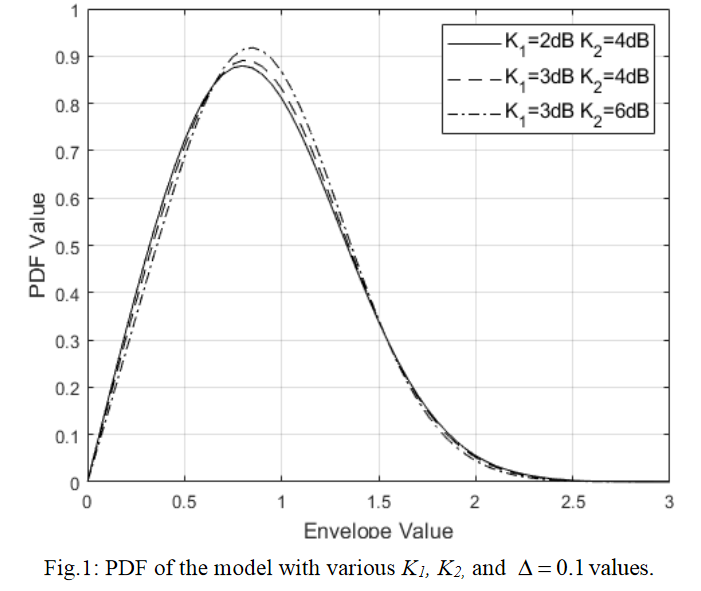
\includegraphics[width=0.5\columnwidth]{Figures/fig1.PNG}
    \label{fig:my_label}
\end{figure}
In Fig.1 for fixed \(\Delta\)= 0.1, as Rician factor \(K_1\) is increased from \(K_1\)=2dB to \(K_1\)=3dB, there is a significant rise in PDF peak due to  a  drop  in  shadowing  for  fixed  TWDP  factor \(K_2\)=4dB.  Similar effect seen when TWDP factor \(K_2\) is varied from \(K_2\)=4dB  to  \(K_2\)=6dB  at  fixed  \(K_1\)=3dB. i.e more LOS component leads to stronger signals
\end{block}
\end{frame}
\begin{frame}
    \begin{block}{Graph 2}
     \begin{figure}
    \centering
    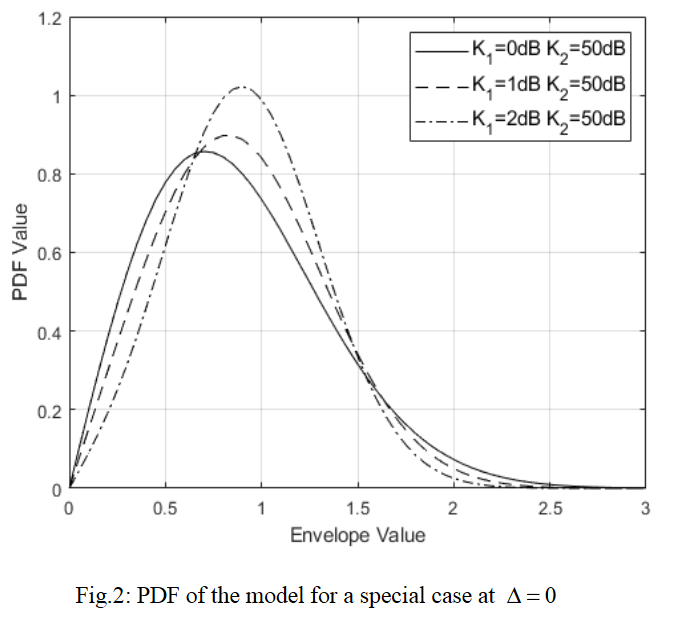
\includegraphics[width=0.5\columnwidth]{Figures/fig2.PNG}
    \label{fig:my_label}
\end{figure}
The  curves  resemble  the  special  case  of  Rayleigh  and  Rician  distribution  when  \(K_2\)   made  very  high  (shadowing  disappears  completely) and \(\Delta=0\), as shown in Fig. 2. At \(K_1\) =0, it behaves as Rayleigh(no LOS component) and for other values it acts as Rician.
\end{block}
\end{frame}
\begin{frame}{}
   \begin{block}{Graph3}
   \begin{figure}
    \centering
    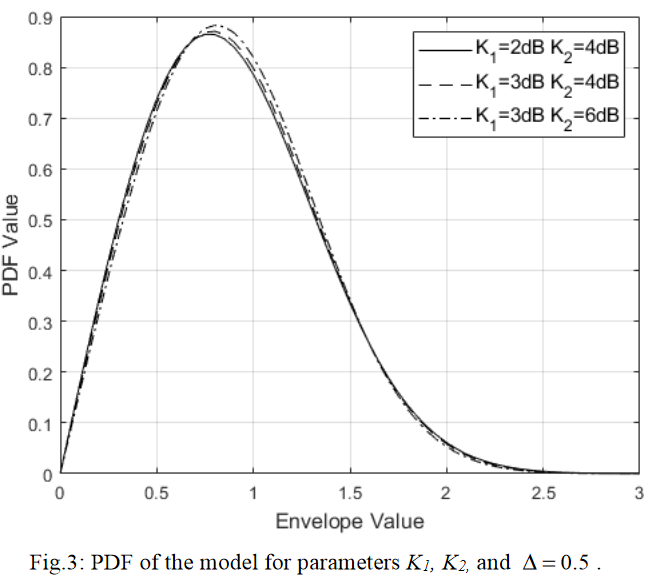
\includegraphics[width=0.5\columnwidth]{Figures/fig3.PNG}
    \label{fig:my_label}
\end{figure}
In Fig. 3 the PDF  is  plotted  for \(\Delta=0.5\) value and it is clearly observed in comparison to Graph 1 that as \(\Delta\) value   increases,   the   peak   density   level   decreases   gradually. i.e One LOS component is better than two.
\end{block} 
\end{frame}
\begin{frame}{}
\begin{block}{Graph 4}
     \begin{figure}
         \centering
         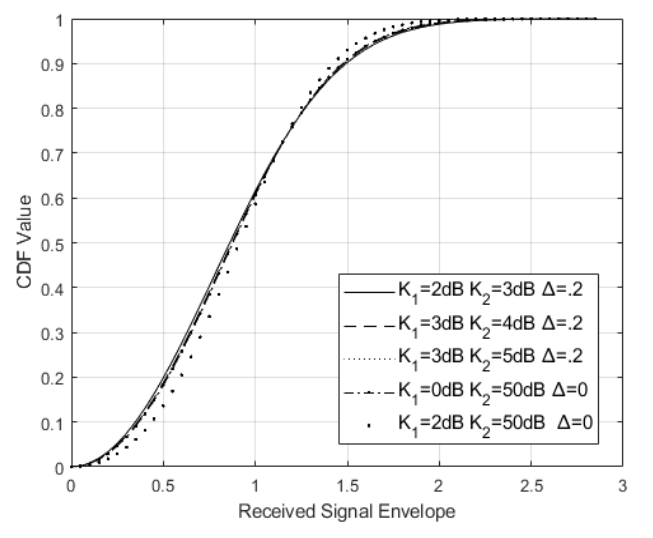
\includegraphics[width=0.5\columnwidth]{Figures/fig4.PNG}
         \caption{Fig.4: CDF of the model for parameters \(K_1\), \(K_2\), and \(\Delta\) values.}
     \end{figure}
\end{block}
The  CDF  of  the  Rician  TWDP  shadowed  fading  model  with  \(\Delta\)=0.2  value  is  shown  in  Fig.4    ,we can see that the pure rician case (\(K_1=0dB,K_2=50dB,\Delta=0\)) performs better than the rest
\end{frame}
\begin{frame}
    \begin{block}{Graph 5}
     \begin{figure}
         \centering
         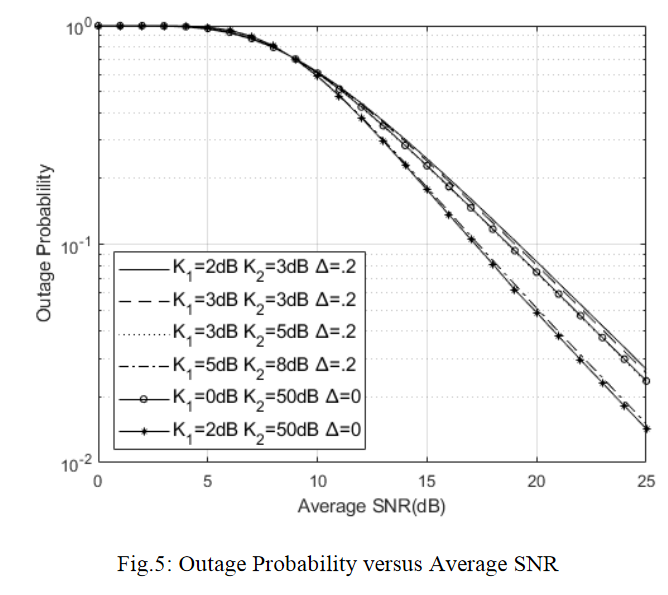
\includegraphics[width=0.5\columnwidth]{Figures/fig5.PNG}
         \label{fig:my_label}
     \end{figure}
     Fig.5  shows  the  graph  of  outage  probability  w.r.t  average  SNR  at  fixed \(\gamma_{th}\)=10dB and \(\Delta\) =0.2.this shows that OP curve decreases quicker for higher values of \(K_1\) and \(K_2\).Special cases also shown with pure rician being best performing curve.
\end{block}
\end{frame}
\end{document}